\section{Sketching and Paper Prototyping}

    \subsection{Sketching}
        For Sketching our team met every Monday and Tuesday to discuss our ideas. Everyone had time to present and the opportunity to share his ideas with the team. After that, we discussed the pros and cons of the ideas and decided which functionalities and aspects we can include in our project.
        
    \subsection{Paper Prototyping}
        For the first draft of the landing page we did a paper prototype. We used some elements from this first drafts to design our layout for Lend'n'Rent.
        
        	\begin{figure}[H]
				\centering
				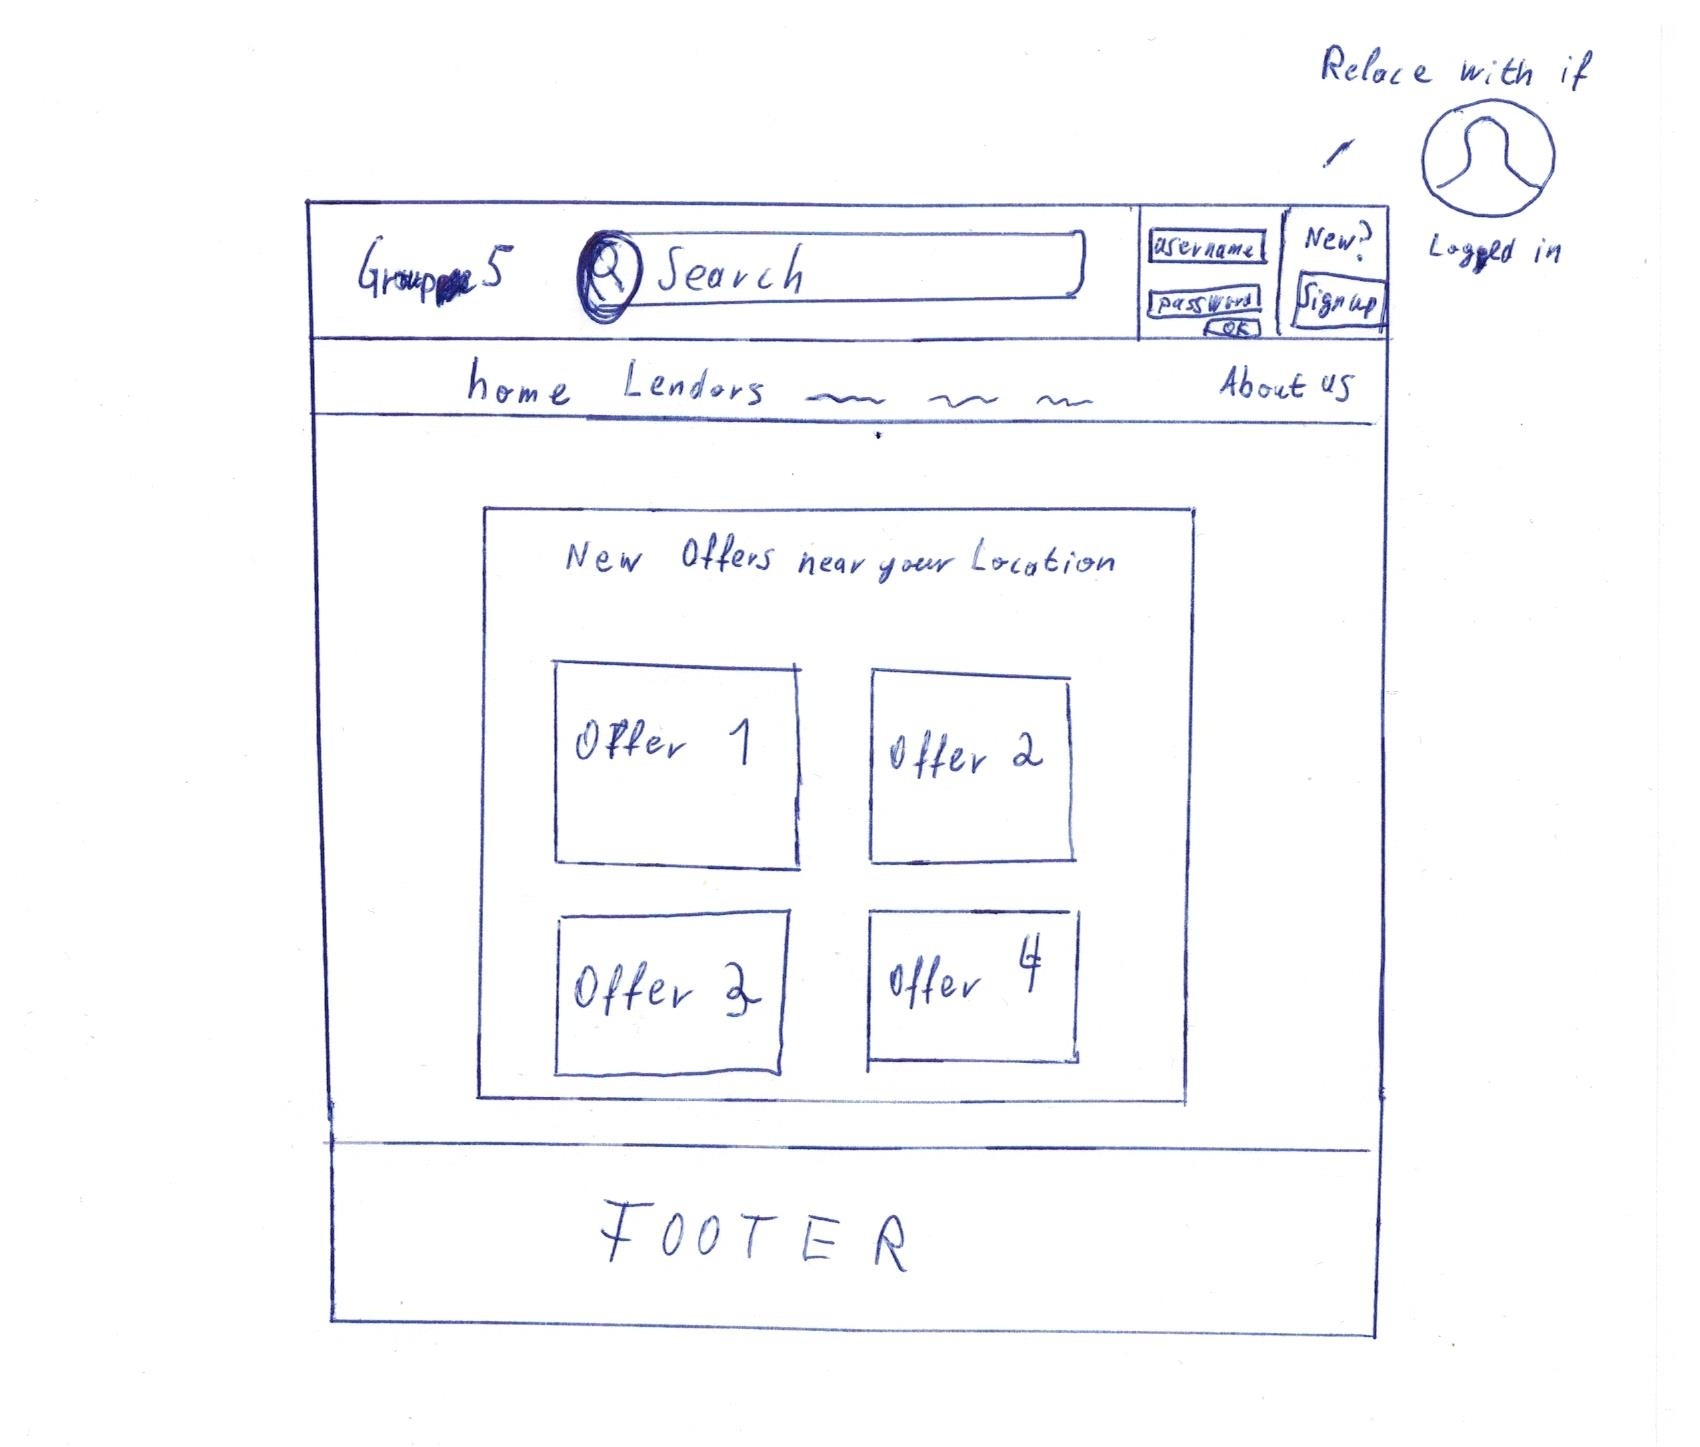
\includegraphics[width=\linewidth]{abb/6_Sketching and Paper Prototyping/Homepage1.png}
				\caption{Landing Page Paper Prototype 1}
				\label{fig:Homepage1}
			\end{figure}
			
			\noindent
			From the first Paper Prototype we take over that the search bar and the Profile picture are included in the navigation bar on top of the website. The Offers we worked into the categories page. 
			
			
			 \begin{figure}[H]
				\centering
				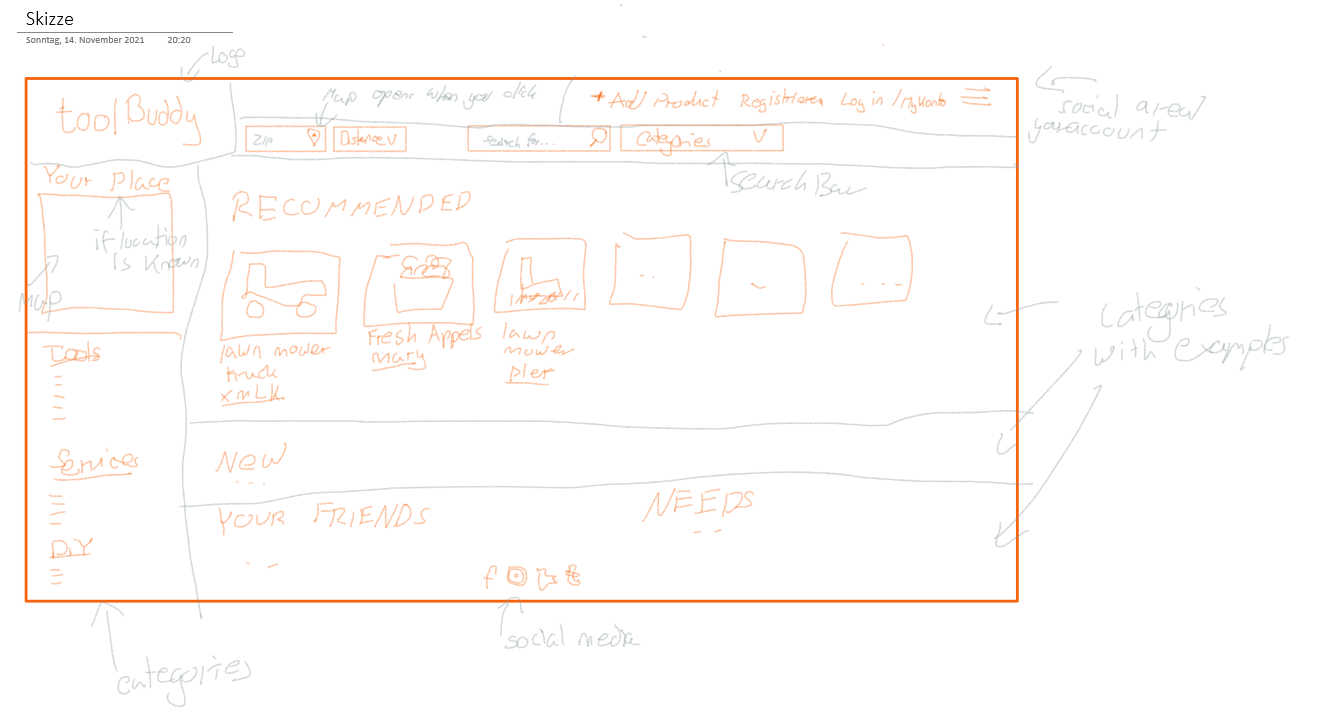
\includegraphics[width=\linewidth]{abb/6_Sketching and Paper Prototyping/Homepage2.png}
				\caption{Landing Page Paper Landing Page 2}
				\label{fig:Homepage2}
			\end{figure}
			
			\noindent
			From Prototype 2 we taken over the left sidebar for the majority of our page flow including the functionality to use a map to look for tools around your area instead using a formula where you need to type your location.
			
			\begin{figure}[H]
				\centering
				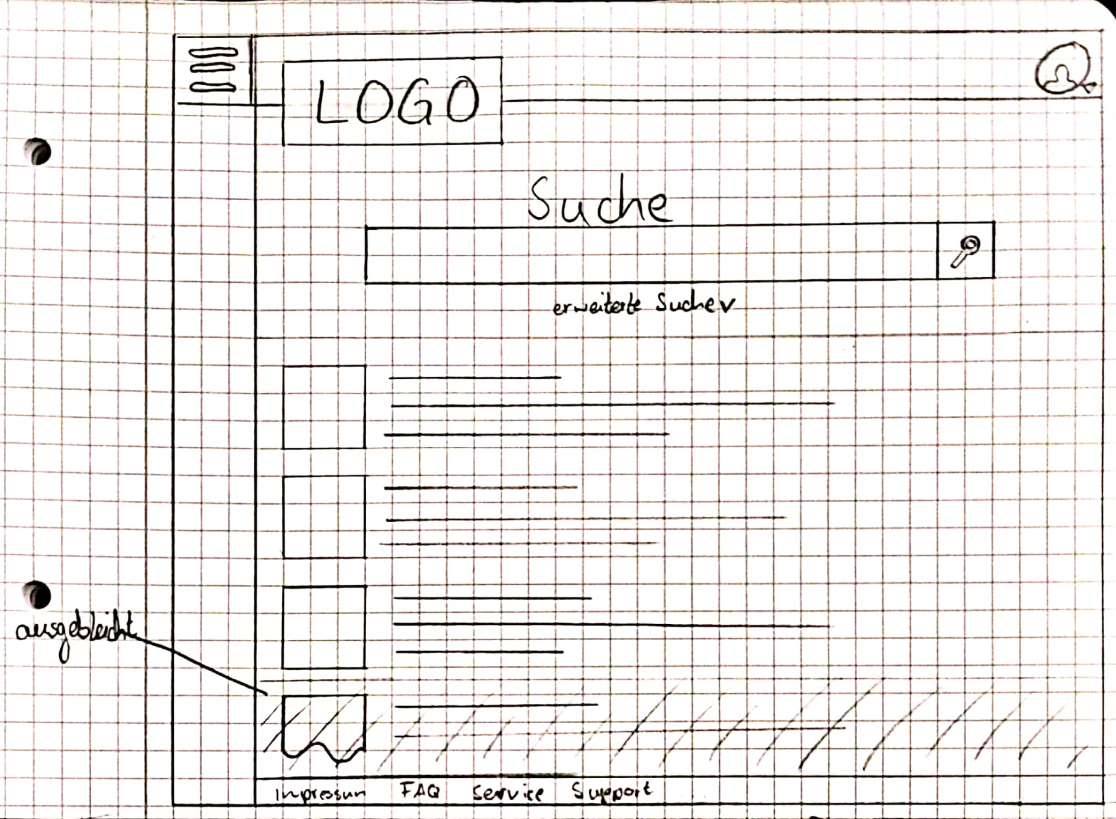
\includegraphics[width=\linewidth]{abb/6_Sketching and Paper Prototyping/Homepage3.png}
				\caption{Landing Page Paper Prototype 3.1}
				\label{fig:Homepage3}
			\end{figure}
			
			
			\begin{figure}[H]
				\centering
				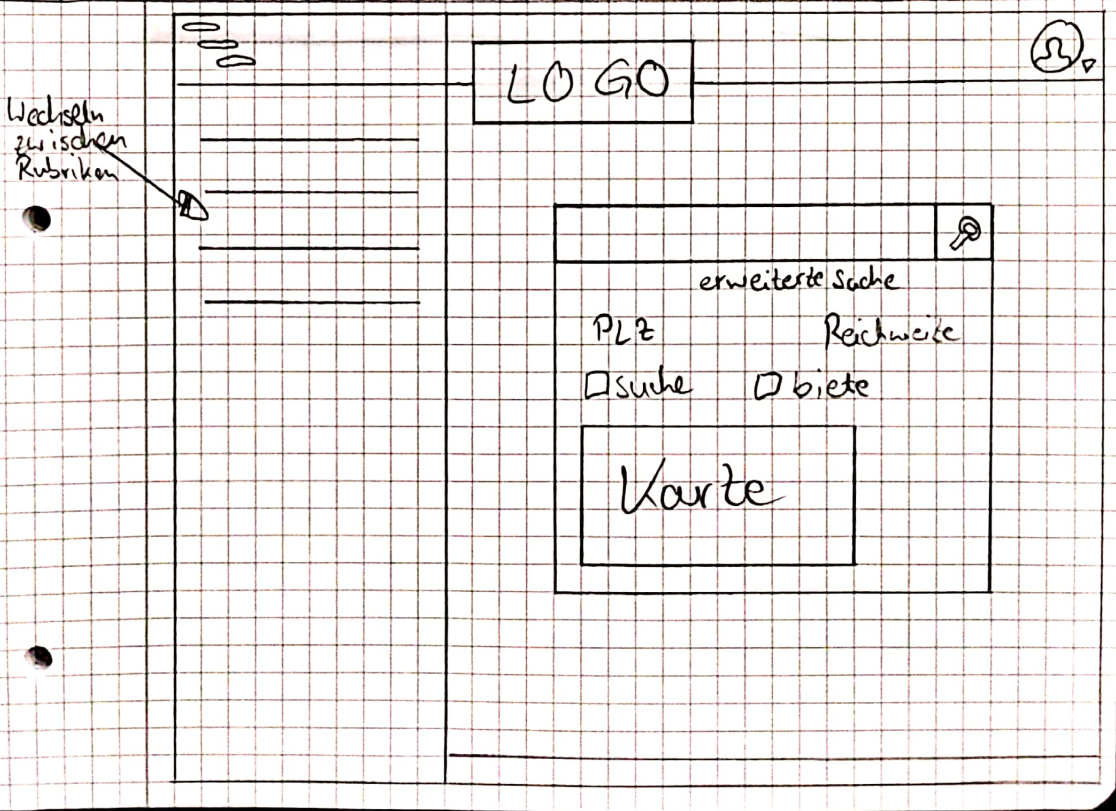
\includegraphics[width=0.9\linewidth]{abb/6_Sketching and Paper Prototyping/Homepage4.png}
				\caption{Landing Page Paper Prototype 3.2}
				\label{fig:Homepage4}
			\end{figure}
			
			\noindent
			From the Prototype 4 we decided to use the arrow under the profile picture to allow user to open a drop down menu for easier navigation.
			
			\begin{figure}[H]
				\centering
				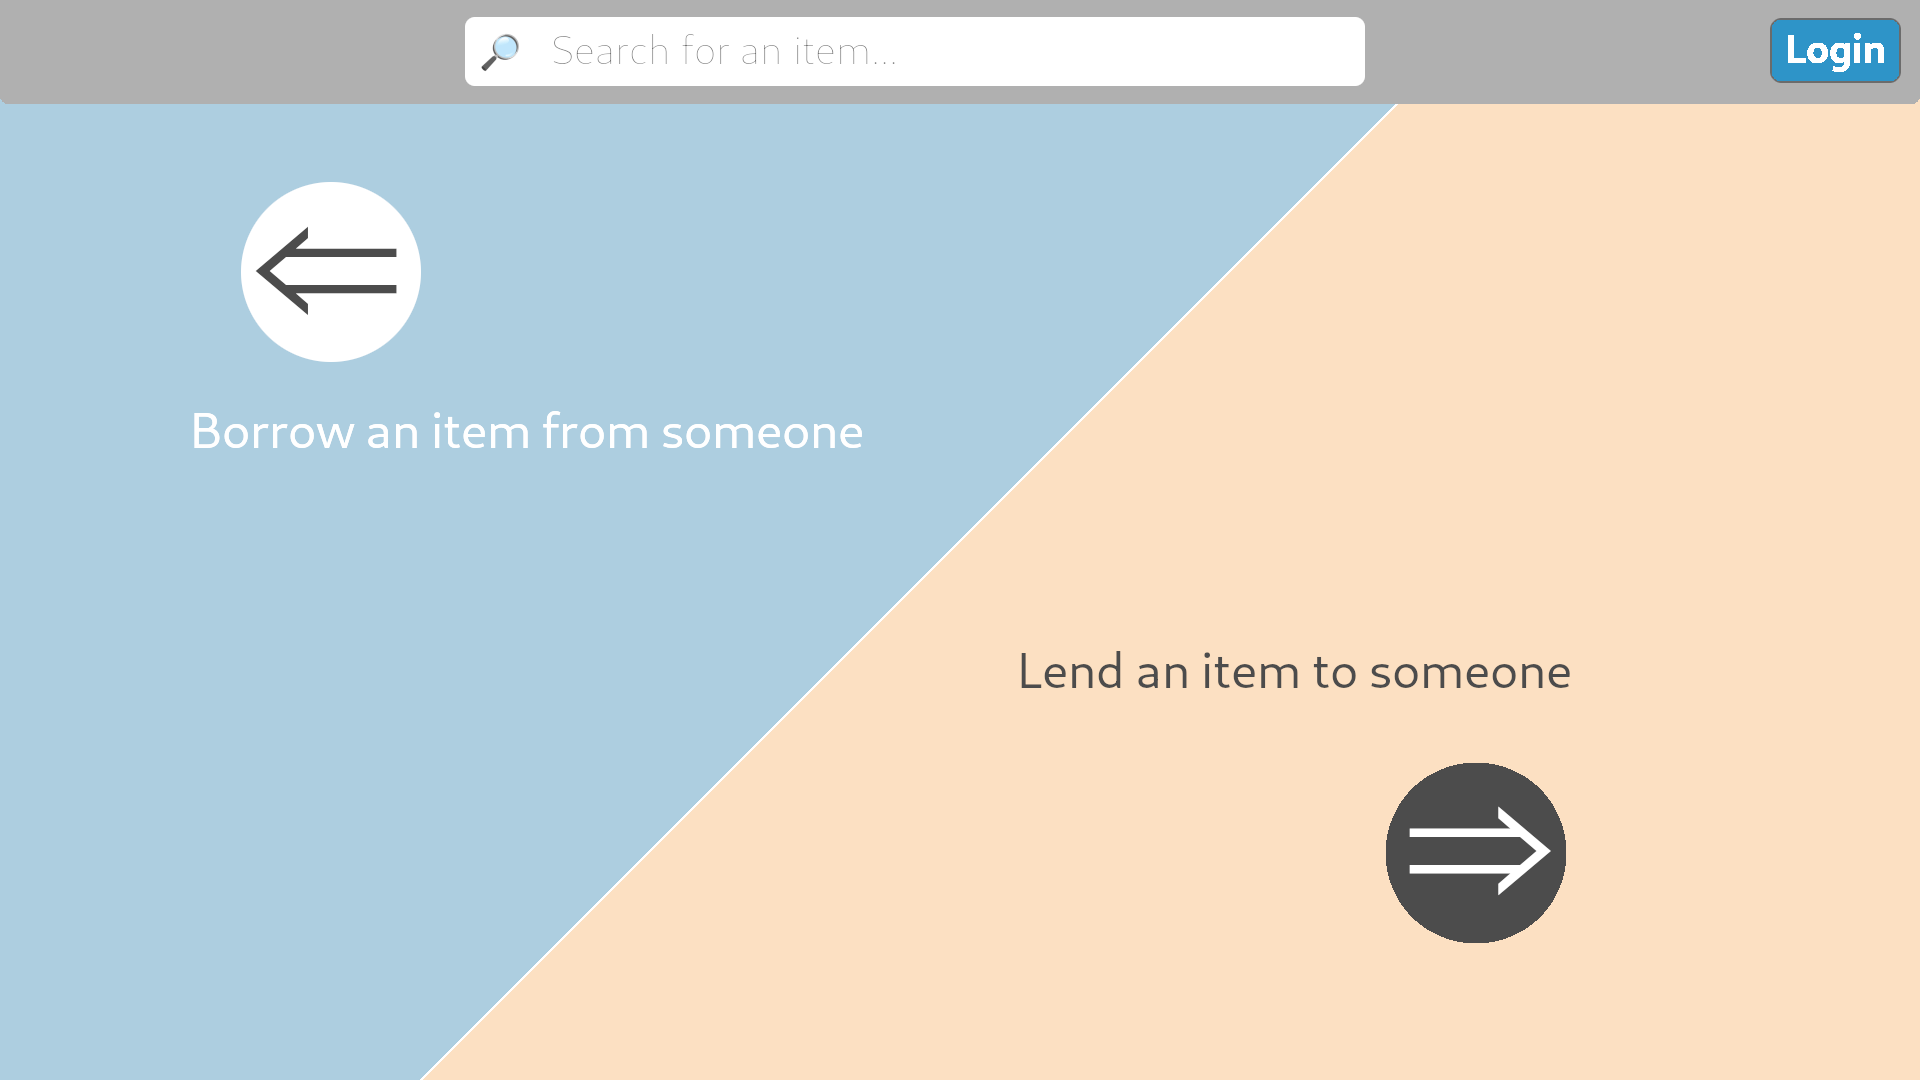
\includegraphics[width=\linewidth]{abb/6_Sketching and Paper Prototyping/Homepage5.png}
				\caption{Landing Page Paper Prototype 4}
				\label{fig:Homepage4}
			\end{figure}
			
			\noindent
			This prototype shows our idea to separate our page flow for our two user groups: Lender and Renter.
			